\documentclass[pdflatex,sn-mathphys-num]{sn-jnl}

\usepackage{graphicx}
\usepackage{amsmath,amssymb}
\usepackage{xcolor}
\usepackage{booktabs}
\usepackage{tabularx}
\usepackage{array}

\raggedbottom

\begin{document}

\title[From greenness to function]{From greenness to function in ecosystem monitoring: continuous trait observables for detecting and attributing climate-driven functional change}

\author*[1]{\fnm{Chaonan} \sur{Ji}}\email{chaonan.ji@ens-paris-saclay.fr}

\author[2]{\fnm{Hannes} \sur{Feilhauer}}\email{hannes.feilhauer@uni-leipzig.de}

\author[2]{\fnm{Eya} \sur{Cherif}}

\author[2]{\fnm{David} \sur{Montero}}

\author[3]{\fnm{Meredith} \sur{Schumann}}

\author[2]{\fnm{Julia} \sur{Joswig}}

\author[4]{\fnm{Ran} \sur{Wang}}

\author[5]{\fnm{Akpona} \sur{Okujeni}}\email{akpona.okujeni@gfz.de}

\author[1]{\fnm{Gabriele} \sur{Facciolo}}\email{gabriele.facciolo@ens-paris-saclay.fr}

\author[6]{\fnm{Philippe} \sur{Ciais}}\email{philippe.ciais@lsce.ipsl.fr}

\author[2]{\fnm{Miguel D.} \sur{Mahecha}}\email{miguel.mahecha@uni-leipzig.de}

\affil*[1]{\orgname{ENS Paris-Saclay}, \orgaddress{\country{France}}}

\affil[2]{\orgname{Leipzig University}, \orgaddress{\city{Leipzig}, \country{Germany}}}

\affil[3]{\orgname{University of Zurich}, \orgaddress{\city{Zurich}, \country{Switzerland}}}

\affil[4]{\orgname{University of Nebraska--Lincoln}, \orgaddress{\city{Lincoln}, \country{USA}}}

\affil[5]{\orgname{GFZ German Research Centre for Geosciences}, \orgaddress{\city{Potsdam}, \country{Germany}}}

\affil[6]{\orgname{Laboratoire des Sciences du Climat et de l'Environnement (LSCE), IPSL}, \orgaddress{\country{France}}}

\abstract{
Climate change is no longer just changing how much vegetation grows: it is changing how vegetation functions. Yet most satellite monitoring still relies on greenness indices and broadband reflectance that detect whether canopies brown or recover, but rarely tell us whether photosynthetic capacity, water status, leaf economics or nutrient regulation have shifted, or whether apparent recovery reflects functional recovery. As climate-impact attribution becomes central to climate-change science, this functional opacity is a measurement bottleneck. Here we argue that ecosystem monitoring should be built around continuous functional observables: spatially and temporally explicit estimates of plant functional traits, anchored in imaging spectroscopy, carried by dense multispectral archives, and complemented by active structural observations from LiDAR, SAR and InSAR. Imaging spectroscopy from PRISMA, EnMAP, EMIT and the upcoming CHIME and SBG missions enables physically interpretable trait retrieval but offers only sparse temporal sampling. Sentinel-2 and Landsat-era archives can transform sparse trait snapshots into continuous trait time series, distinguishing resistance, recovery and legacy effects at scales relevant to attribution and management. We propose a framework distinguishing directly observed, spectrally anchored, ecologically inferred, climate-context inferred and structurally complemented information, with six principles for credible functional observables. A European forest illustration shows trait-specific feasibility and failure modes. The framework offers a path from describing greenness change to attributing functional change in a warming world.
}

\keywords{functional observables, imaging spectroscopy, hyperspectral remote sensing, multispectral time series, plant traits, ecosystem monitoring, vegetation resilience}

\maketitle

\section{Greenness is not enough}

Climate change is no longer just changing where and when vegetation grows; it is changing how vegetation functions. Heatwaves, multi-year droughts and compound climate extremes drive distinct functional responses across global forests, grasslands and croplands -- altering pigment composition, water regulation, leaf economics and nutrient status before, during and after the events that satellites currently detect as greenness anomalies \cite{ipbes2019,seidl2017,forzieri2022mortality,smith2022resilience,mahecha2024biodiversity}. Distinguishing these functional responses is becoming central to climate-impact attribution: a brown canopy after a heatwave may reflect photosynthetic shutdown, water limitation, pigment stress or defoliation, and apparent recovery in greenness can hide altered leaf economics or nutrient regulation. Monitoring systems that cannot resolve these dimensions risk underestimating the functional consequences of climate extremes for ecosystem services, carbon balance and resilience.

Satellite remote sensing has transformed the spatial scale and temporal continuity of ecosystem observation \cite{pettorelli2018satellite,balsamo2018satellite}. Sentinel-2 and Landsat-era archives now provide two decades of vegetation memory that field campaigns alone cannot match. Yet many operational products still rely on optical vegetation indices or broadband reflectance summaries. These indicators are indispensable for detection, but they are not direct ecological state variables. Sun-induced chlorophyll fluorescence (SIF) and near-infrared reflectance of vegetation (NIRv) have added partial functional capability by linking observations more directly to photosynthetic activity \cite{sun2017oco2sif,badgley2017nirv}, yet they remain integrative proxies that cannot identify which trait dimensions of canopy function have changed. Similar spectral or fluorescence trajectories can arise from very different combinations of canopy structure, pigment concentration, water limitation, phenology, viewing geometry and species composition. This ambiguity matters because climate-attribution science increasingly requires not detection alone, but the diagnosis of which functional pathway responded, when, and how persistently \cite{zeng2022optical,yan2025forestrecovery}.

The next step is therefore not simply higher spatial resolution or more frequent images. It is the construction of continuous, interpretable functional observables. Plant functional traits offer a particularly promising route, because traits such as leaf area index (LAI), chlorophyll content, nitrogen, leaf mass per area (LMA), equivalent water thickness and lignin connect remote observations to photosynthesis, water regulation, nutrient status, leaf economics and carbon turnover. Decades of trait ecology---from the leaf economics spectrum \cite{wright2004leafeconomic} to global functional gradients \cite{diaz2016global}---have shown that such variables organize plant strategies and ecosystem responses to environmental forcing. Trait-based monitoring would allow remote sensing products to be interpreted in terms of changing ecosystem function rather than only changing spectral appearance, consistent with the broader emergence of spectral biology and plant functional-diversity monitoring from space \cite{jetz2016monitoring,Schweiger2018,schweiger2022beta,cavender2025spectral}.

The challenge is that no current observing system solves this problem alone. Field trait networks are ecologically rich but spatially sparse. Multispectral satellites are temporally dense but spectrally limited. SIF and NIRv contribute information about photosynthetic activity but not about which trait dimensions of canopy function have changed. Imaging spectroscopy is information-rich but temporally sparse. LiDAR, SAR and InSAR provide stronger constraints on canopy structure than passive optical spectra, but do not directly deliver biochemical traits. The opportunity is to treat these systems as complementary parts of one ecological measurement system.

This Perspective makes three claims. First, greenness-based monitoring is indispensable for detection but insufficient for diagnosing functional change, particularly under the climate-impact attribution demands that increasingly shape ecological and climate science. Second, imaging spectroscopy should be understood as an essential trait-retrieval technology and as a source of functional anchors for monitoring. Third, dense multispectral archives can provide the temporal carrier needed to transform sparse trait snapshots into continuous, uncertainty-aware functional observables. The novelty is not another review of hyperspectral retrieval methods. It is the shift from trait snapshots to functional time series: from retrieving traits at observation times to building ecological monitoring variables for stress attribution, recovery assessment, legacy-effect analysis and Earth-system model evaluation in a warming world.

\begin{figure}[t]
\centering
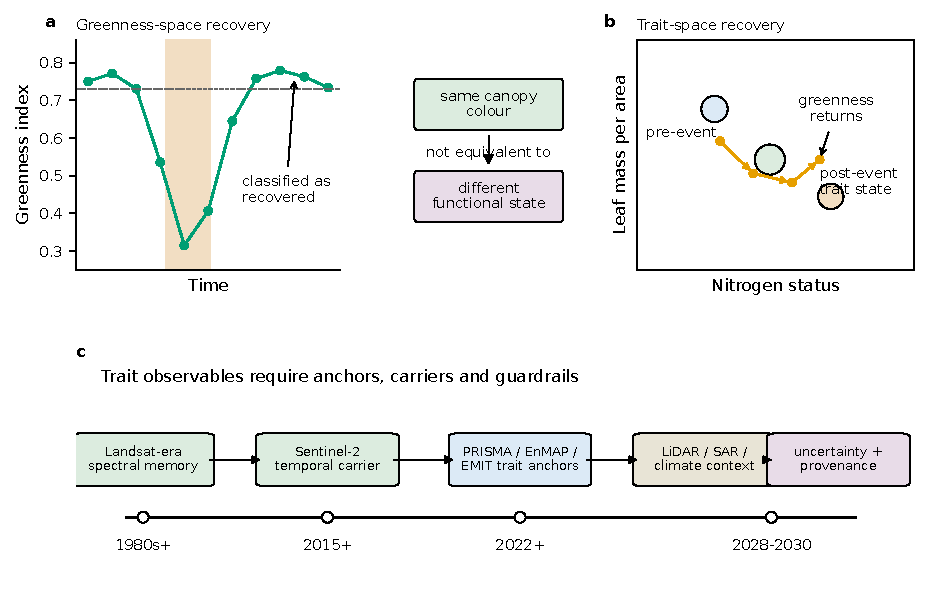
\includegraphics[width=\textwidth]{figures/generated/fig1_from_trait_snapshots_to_functional_time_series.pdf}
\caption{\textbf{From trait snapshots to functional time series.} Spectral-index and multispectral archives provide the temporal memory needed for long-term monitoring, while imaging spectroscopy provides functional specificity by retrieving biochemical and optical trait anchors. Future CHIME/SBG-class observations will increase hyperspectral coverage, but long-term ecosystem monitoring also requires densifying sparse trait retrievals and reconstructing trait-relevant functional states through existing Sentinel-2 and Landsat-era archives. LiDAR, SAR and InSAR provide complementary structural constraints, and each product should carry uncertainty, provenance and domain-of-applicability information.}
\label{fig:trait_snapshots_time_series}
\end{figure}

\section{Imaging spectroscopy makes function observable, but not continuous}

Imaging spectroscopy matters because it records narrow, contiguous spectral bands that are sensitive to canopy optical properties, pigments, water absorption features and biochemical composition. It can also carry indirect information about canopy state because structure modulates reflectance, but it should not be treated as a direct three-dimensional structure sensor. Canopy height, vertical complexity, woody volume and related structural variables are more directly constrained by active remote sensing, particularly LiDAR, SAR and InSAR \cite{dubayah2024structural,lang2024gedi}. Spectral information can be translated into plant traits through empirical models, radiative transfer model inversion, hybrid physical-statistical approaches or machine learning. Multi-trait retrieval studies have shown that heterogeneous spectral and trait datasets can support transferable models for a suite of plant functional traits \cite{cherif2023spectra}. Curated community datasets and trait databases provide an expanding foundation for this work \cite{kattge2020try,mederer2025plant,wu2026gsti}.

Recent work also clarifies the limits of this promise. Transferability is not automatic. Models trained on one species set, plant functional type, season or region may fail elsewhere if the calibration domain does not cover the trait range, canopy structure or atmospheric conditions of application. Studies by Fujiang Ji and colleagues are useful here as objective field evidence, not as results from the European forest illustration described below. Their work on spectral-trait model transferability highlights that calibration diversity and domain awareness are central constraints for leaf trait estimation \cite{ji2024transferability}. Related transfer-learning approaches that combine radiative transfer model knowledge with field observations show how generalization may be improved \cite{ji2025transferlearning}. At canopy scale, recent PRISMA and NEON analyses indicate that spaceborne imaging spectroscopy can track seasonal variability in multiple plant traits across sites \cite{ji2025prisma}. Together, these studies suggest that the trait-anchor problem is becoming increasingly tractable, even though temporally continuous monitoring remains unresolved.

Together, these studies establish a boundary condition for this Perspective: trait retrieval is an active and essential capability, but not a solved operational service. It is improving rapidly and still requires explicit attention to calibration domain, scale and uncertainty. That middle position is important. Overstating retrieval reliability would make the functional-monitoring argument technologically naive; understating recent progress would make the proposed monitoring framework appear premature.

This distinction is important for the framing of this Perspective. Robust retrieval from imaging spectroscopy remains a core research task, especially as PRISMA, EnMAP, EMIT, CHIME and the Surface Biology and Geology mission expand the observational basis for vegetation functional traits \cite{chabrillat2024enmap,nieke2018towards,cawse2021nasa}. The additional monitoring question is how those retrievals can be embedded into continuous ecological time series. Revisit frequency, clouds, tasking strategies and the short historical archive mean that hyperspectral imagery alone will not provide multi-decadal trait time series for most ecosystems.

The highest ecological value of imaging spectroscopy may therefore be as a functional anchor. It can define what should be monitored: a set of physiologically interpretable traits with physical units and ecological meaning. Dense multispectral archives can then provide the temporal support needed to follow those variables between sparse hyperspectral observations. Section 7 returns to the timing of this transition in the context of the upcoming CHIME and SBG missions.

\section{From trait snapshots to functional time series}

\noindent\fbox{%
\begin{minipage}{0.94\textwidth}
\textbf{Definition.} A \textit{continuous functional observable} is a spatially and temporally explicit estimate of ecosystem function---typically a plant functional trait---that can be interpreted ecologically, compared through time, and evaluated with quantified uncertainty and a documented domain of applicability.
\end{minipage}}

\vspace{0.5em}

This framework operationalizes trait ecology: it translates the leaf-economics and functional-gradient paradigms into a continuous, uncertainty-aware spatiotemporal measurement system that ecological and climate science can act on. In this Perspective, the most important observables are plant functional traits. A trait-based data cube is one implementation of this broader idea: space by time by trait, with enough metadata to evaluate where estimates are reliable and what biological interpretation they support.

\textit{Densification} and \textit{retrospective reconstruction} should be separated. \textit{Densification} refers to filling temporal gaps between sparse hyperspectral trait retrievals within the contemporary satellite record. \textit{Retrospective reconstruction} refers to cautious inference of trait-relevant functional states through existing multispectral archives, especially Sentinel-2 since 2015 and, trait by trait where defensible, Landsat-era records extending back through past decades. This distinction is not merely terminological: it determines which traits can be reported with calibrated uncertainty during the contemporary EnMAP/PRISMA era versus which require extra-domain assumptions for Landsat-era reconstruction, and therefore which products are credible for climate-impact attribution rather than only descriptive analysis. Future CHIME and SBG observations will make trait snapshots more systematic, but they will not remove the need to connect those snapshots with the historical monitoring record.

Not all target traits have the same relationship to imaging spectroscopy. Some traits are closer to the spectral measurement, because they influence absorption or scattering features more directly. Others are inferred partly through trait covariation, phenological context, canopy state and ecological correlation. This distinction should be explicit. A framework for functional observables should not imply that every trait is directly observed by hyperspectral data. Instead, it should report which traits are spectrally anchored, which are statistically or ecologically inferred, and how uncertainty propagates across those links.

\noindent\fbox{%
\begin{minipage}{0.94\textwidth}
\textbf{Box 1. Observed, anchored, inferred and complemented information.}

\begin{tabularx}{\textwidth}{>{\raggedright\arraybackslash}p{0.24\textwidth}>{\raggedright\arraybackslash}X>{\raggedright\arraybackslash}p{0.24\textwidth}}
\toprule
\textbf{Information class} & \textbf{Examples} & \textbf{Primary constraint} \\
\midrule
Directly observed optical signal & Surface or canopy reflectance, absorption features, spectral shape & Imaging spectroscopy or multispectral sensors \\
Spectrally anchored traits & Pigments, water-related traits, some biochemical and optical traits & Imaging spectroscopy plus field or airborne trait calibration \\
Contextually inferred traits & Nitrogen, LMA, lignin, allocation-related or community-level variables when retrieved through trait covariation and ecological context & Spectral anchors, temporal context, trait covariance and validation data \\
Climate-context inferred & Trait states resolved through reanalysis priors (e.g.~ERA5) and Sentinel-2 phenology when direct spectral anchors are missing or noisy & Climate priors must be flagged in product metadata; uncertainty must inflate when extrapolating beyond training climate domain \\
Complementary structure & Canopy height, vertical complexity, woody volume, biomass-related structure & LiDAR, SAR, InSAR and field inventory data \\
\bottomrule
\end{tabularx}

This distinction is central to credible functional monitoring. A trait product should state whether a variable is directly observed, spectrally anchored, inferred through ecological or statistical relationships, or constrained by a complementary sensor.
\end{minipage}}

There are two possible routes from sparse imaging spectroscopy to such observables. One route is to reconstruct full hyperspectral imagery from multispectral and hyperspectral fusion. This is an active and valuable research area \cite{yokoya2017hyperspectral}. The second route, which we emphasize here, is trait-level reconstruction. For many ecological applications the objective is not to reconstruct spectra themselves, but to reconstruct the functional variables that spectra make observable. Directly modelling traits can reduce dimensionality, avoid a two-step cascade of spectral reconstruction followed by trait retrieval, and produce outputs that ecologists and modellers can interpret more directly.

The distinction is practical as well as conceptual. A full reconstructed hyperspectral cube may be the right target when downstream users need spectra for multiple unknown future applications. Trait-level reconstruction is preferable when the scientific question is already framed in terms of vegetation function, disturbance response, biodiversity monitoring or model constraints. For climate-impact attribution in particular, the functional question is rarely about spectra themselves: it is about which traits---and therefore which functional pathways---have changed, in what sequence and how confidently. In this case, spectra are the measurement pathway rather than the final ecological variable. The model can be trained and evaluated around the traits that matter, and uncertainty can be expressed in the units that users interpret.

Recent Sentinel-2 trait and phenology studies show that multispectral temporal context contains useful trait information \cite{liu2024spectraphenology}; the unresolved challenge is to make such reconstructions explicitly anchored, validated and uncertainty-aware. LiDAR, SAR and InSAR can provide structural covariates where canopy height, vertical complexity or biomass-related information is needed, and climate reanalysis, topography, land cover and disturbance data can provide additional contextual covariates. Models then learn the relationship between temporal multispectral context, structural context where available, and hyperspectral-derived trait labels, while preserving the distinction between observed trait anchors, densified trait estimates and retrospective predictions outside the training domain.

\begin{figure}[t]
\centering
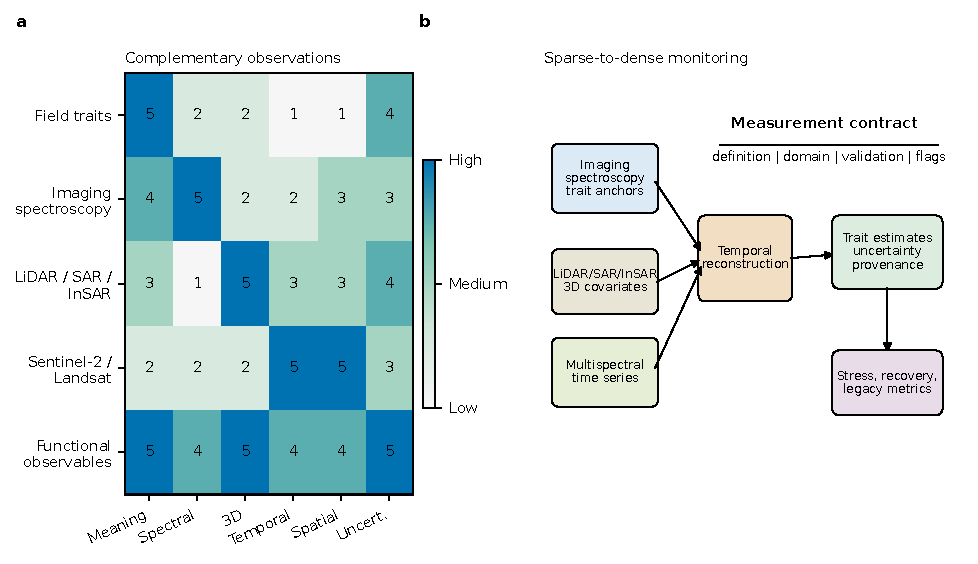
\includegraphics[width=\textwidth]{figures/generated/fig2_functional_observables_framework.pdf}
\caption{\textbf{Sparse-to-dense framework for continuous functional observables.} Field traits, imaging spectroscopy, active structure observations and multispectral time series each solve only part of the monitoring problem. Continuous functional observables combine their strengths by using imaging spectroscopy as a source of biochemical and optical trait anchors, LiDAR/SAR/InSAR as structural covariates where available, dense multispectral records as temporal carriers and an explicit measurement contract that records trait definitions, training domain, validation design, uncertainty and provenance.}
\label{fig:framework}
\end{figure}

Such models should be evaluated as ecological measurement systems, not only as prediction algorithms. A useful functional-observable product must report its training domain, sensor inputs, temporal window, trait definitions, validation design and uncertainty. It should also distinguish interpolation from extrapolation. A model applied to a new site, a new drought regime or a different canopy type should not silently produce the same type of estimate as a model applied within its calibration domain.

This measurement-system framing also changes how model complexity should be judged. A deep model may improve performance if it captures temporal structure and multimodal context, but a simpler model may be preferable if it is more stable, easier to validate and more transparent about domain limits. For a Perspective aimed at ecology and climate science audiences, the central point is not to advocate a particular architecture. It is to argue that the model layer should be subordinate to the ecological measurement contract: the trait definition, the temporal support, the uncertainty estimate and the validation design. In a climate-attribution framing, the uncertainty estimate is not a methodological footnote: it is the decisive input to whether a detected trait anomaly can be attributed to a climate driver, or whether it remains within the product's own noise floor.

\section{A European forest illustration of trait-specific feasibility}

To illustrate how the framework above can be implemented and judged, we draw on a compact European forest example. \textbf{This is a design illustration, not an operational benchmark.} It is meant to expose where the framework succeeds and where it exposes failure modes that themselves justify the principles in Box 4. A complete benchmark with all 20 traits, cross-site generalization, calibrated uncertainty and event case studies belongs in companion research papers.

This framing protects the manuscript from overclaiming. The illustration need not prove that operational trait monitoring is solved. It only needs to show that the observing strategy can be implemented with present Earth observation archives and judged by ecological criteria. The useful message is not that every trait is already reconstructed well; it is that functional observables can be built, tested and reported honestly, and that trait-specific failure modes are themselves diagnostic information that climate-attribution users need.

\noindent\fbox{%
\begin{minipage}{0.94\textwidth}
\textbf{Box 2. Where trait illustration meets the framework.}

Our testbed links hyperspectral-derived trait labels (EnMAP, with PRISMA as a complementary source) with Sentinel-2 temporal observations across European forest sites. The broader analysis targets 20 traits; this Perspective highlights five illustrative traits: LAI, chlorophyll, nitrogen, LMA and lignin. These traits should \textit{not} be interpreted as equally direct spectral measurements: chlorophyll and water-related traits are closer to specific optical absorption features; nitrogen, LMA and lignin are often supported by broader spectral information and trait covariation; LAI is a canopy state variable, not a substitute for active measurements of three-dimensional structure. The illustration shows that sparse-to-dense functional monitoring can be implemented and evaluated trait by trait. Results are strongest for LAI, intermediate for LMA, nitrogen and lignin, and weaker for chlorophyll. \textit{This trait-specific patterning is not a methodological weakness---it is the framework's intended readout}: a continuous functional observable must report differentiated, trait-specific skill rather than a single average accuracy, because that is what climate-attribution science actually requires from a monitoring product.
\end{minipage}}

\begin{figure}[t]
\centering
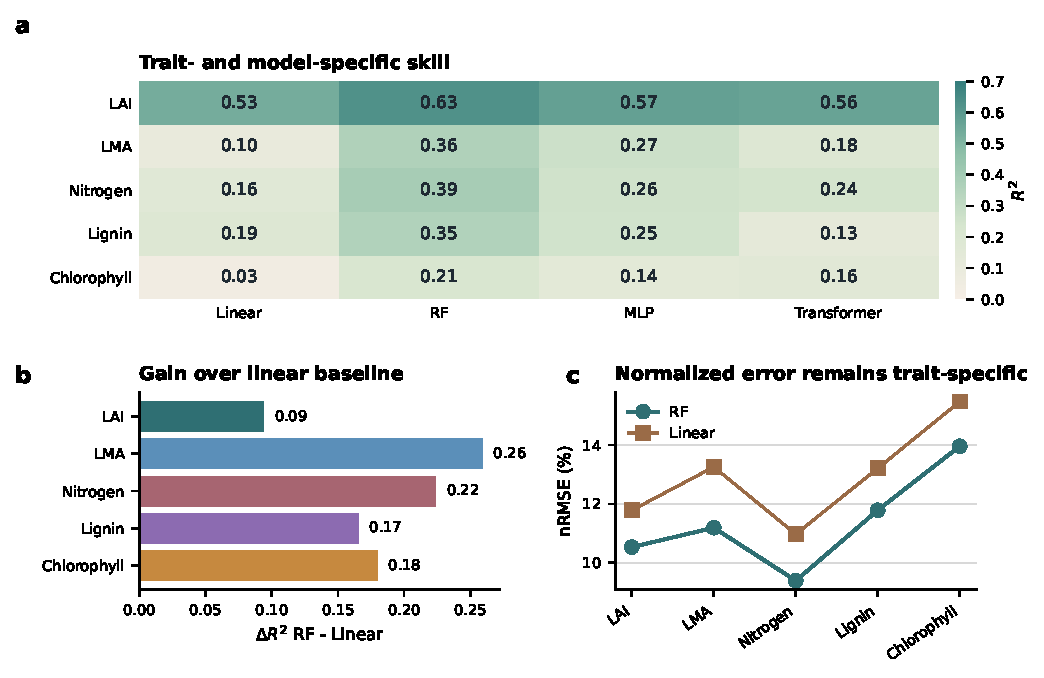
\includegraphics[width=\textwidth]{figures/generated/fig3_proof_of_concept_performance.pdf}
\caption{\textbf{Illustrative trait-specific readout under the proposed framework.} Early common-test evaluation for five hyperspectral-derived traits reconstructed from Sentinel-2 temporal context in a European forest testbed. \textbf{a--c}, Trait-specific predictive skill, normalized error and the gain of a non-linear baseline over a linear baseline; results are strongest for LAI, intermediate for LMA/nitrogen/lignin, and weaker for chlorophyll. \textbf{d}, Schematic of the intended time-series product: sparse trait anchors, densified estimates, uncertainty bands and domain-of-applicability flags. The trait-by-trait variation in skill is itself part of the framework's intended output: a continuous functional observable must report not a single accuracy number, but a trait-specific readiness map that downstream users---especially climate-attribution and policy users---can act on. These panels are illustrative, not an operational benchmark. \textit{[Author note: panels a--c may be re-rendered as a traffic-light readiness matrix in a later revision; current placeholder retains numerical heatmaps until the figure regeneration is run.]}}
\label{fig:proof_of_concept}
\end{figure}

\section{What continuous functional observables enable for climate science}

Continuous functional observables change the type of ecological question that can be asked from space. Greenness anomalies are useful but often descriptive. Trait anomalies can be process-oriented. A decline in greenness during drought, for example, may reflect pigment degradation, leaf area loss, canopy water limitation, phenological transition, or a mixture of these processes. Trait time series allow these pathways to be separated more explicitly by examining the joint dynamics of pigments, water-related traits, leaf economics and canopy structure. This is where existing greenness archives and new trait observations become mutually reinforcing: the archive supplies historical continuity, while trait anchors improve the functional interpretation of that continuity.

\subsection{Stress syndromes: trait fingerprints of climate impact}

The first opportunity is the identification of stress syndromes. Ecosystem stress rarely acts through a single variable. Drought may alter water content, stomatal regulation, pigment protection, LAI and LMA. Nutrient limitation may affect nitrogen and chlorophyll without immediately changing canopy area. Heat damage may affect pigments and photosynthetic capacity before structural loss is visible. Trait combinations therefore provide a richer diagnostic space than single spectral indices. A functional-observable framework does not simply ask whether vegetation became greener or browner. It asks which functional dimensions changed, in what sequence and under which environmental context.

The term syndrome is useful because no single trait should be expected to diagnose every stressor. In many ecosystems, stress responses are mixtures of short-term physiological adjustment, seasonal development and longer-term structural change. A chlorophyll anomaly without an LAI anomaly may suggest a different process than a simultaneous decline in both. A water-related anomaly followed by delayed structural decline may imply a different trajectory than an abrupt canopy loss. Trait time series make it possible to formulate such hypotheses consistently across sites and events, even when final attribution still requires climate, management and field context.

\noindent\fbox{%
\begin{minipage}{0.94\textwidth}
\textbf{Box 3. Hypothesized trait fingerprints of common climate stressors.}

\begin{tabularx}{\textwidth}{>{\raggedright\arraybackslash}p{0.22\textwidth}>{\raggedright\arraybackslash}X}
\toprule
\textbf{Climate stressor} & \textbf{Expected trait fingerprint (illustrative; not exhaustive)} \\
\midrule
Soil drought & $\downarrow$ equivalent water thickness, then $\downarrow$ pigments, $\uparrow$ LMA; eventual $\downarrow$ LAI if drought persists \\
Heatwave (short, intense) & $\downarrow$ photosynthetic pigments, potential $\uparrow$ photoprotective pigments before structural loss \\
Compound drought--heat & Combined water and pigment signatures; legacy in LMA and nitrogen even after greenness recovery \\
Nutrient limitation & $\downarrow$ nitrogen, $\downarrow$ chlorophyll, with canopy structure largely preserved \\
Biotic outbreak (e.g.~bark beetle) & Spatially clustered $\downarrow$ LAI with altered structural metrics; pigments may decline late \\
\bottomrule
\end{tabularx}

These fingerprints are hypotheses to be tested with continuous functional observables and field validation. The point is not that they are universal, but that they are testable---unlike the single-index anomalies on which much climate-impact attribution still relies.
\end{minipage}}

\subsection{Resistance, recovery and legacy effects after climate extremes}

The second opportunity is event-oriented monitoring. Extreme events are often evaluated using deviations from a baseline, but the chosen observable strongly affects interpretation. Trait time series allow resistance to be quantified as the functional deviation during disturbance, recovery as the trajectory back towards a pre-event state, and legacy effects as persistent trait offsets after apparent recovery. A canopy may recover greenness while nitrogen, water status or leaf economics remain altered. Conversely, a temporary decline in a structural variable may not imply long-term functional damage if physiological traits recover quickly. Continuous functional observables can therefore support a more mechanistic analysis of droughts, heatwaves, frost events and insect outbreaks.

This is particularly relevant for compound and sequential extremes. A forest stand exposed to spring drought, summer heat and subsequent insect pressure may show a complex temporal signature that is difficult to summarize with one index. Trait time series allow the response to be decomposed into functional dimensions and compared across events. They could also support more informative baselines: not only the expected greenness for a given date, but the expected trait state given phenology, climate and site history. Trait-based legacy detection could complement existing climate-attribution chains (climate forcing $\rightarrow$ ecosystem response $\rightarrow$ impact), giving observation-based constraints on the functional component that current attribution chains often treat as a black box.

\subsection{Dynamic functional diversity and Earth system model evaluation}

The third opportunity is dynamic functional diversity. Trait maps are often summarized by mean values, but ecosystems are composed of trait distributions. If continuous functional observables preserve spatial and temporal heterogeneity, they can be used to monitor changes in functional composition, intraspecific variability and community-level stability. They can also provide empirical constraints for ecosystem and carbon-cycle models that currently rely on plant functional types or static trait parameterizations. In this sense, trait-based observables are not replacements for process models. They are observational state variables that can be used to evaluate whether models reproduce functional responses to environmental forcing.

This point is central for keeping the manuscript ecological rather than technological. Trait-based observables are valuable because they can connect levels of organization: leaves and canopies, pixels and stands, communities and landscapes, observations and models. Their most important products may not be individual trait maps, but derived ecological quantities such as trait anomalies, functional dispersion, stress-syndrome classes and recovery metrics. These derived variables should be treated as hypotheses to be tested against field observations, flux measurements and ecological theory. They are also natural evaluation targets for next-generation Earth system models (CMIP7 and beyond), where plant functional type or static trait parameterizations could increasingly be benchmarked against observation-based dynamic trait fields.

\begin{figure}[t]
\centering
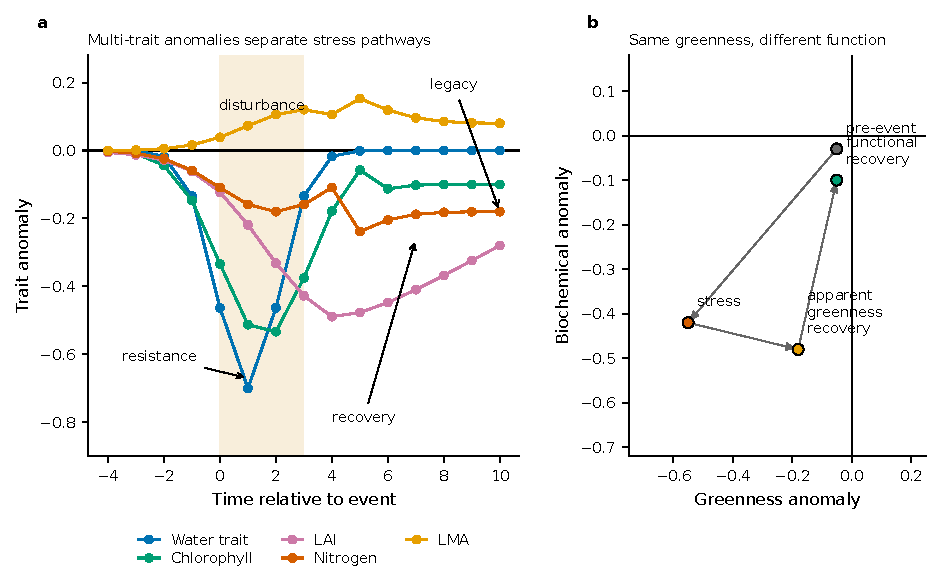
\includegraphics[width=\textwidth]{figures/generated/fig4_trait_anomaly_syndromes.pdf}
\caption{\textbf{Trait fingerprints of climate impact.} Multi-trait time series can separate stress pathways that would be collapsed in a single greenness anomaly. Conceptual trajectories illustrate how water-related traits, chlorophyll, LAI, nitrogen and LMA could respond with different timing, resistance, recovery and legacy effects following climate stressors. The state-space panel emphasizes that apparent greenness recovery need not imply functional recovery, a distinction that matters for climate-impact attribution. \textit{[Author note: figure remains conceptual; could later be partly anchored in a drought/heatwave case study from the European testbed.]}}
\label{fig:anomalies}
\end{figure}

\section{Guardrails: uncertainty, transferability and ecological validation}

Functional observables will only be useful if their uncertainty is treated as part of the product. The first uncertainty layer arises from the hyperspectral trait anchor itself. Trait retrieval models may be affected by atmospheric correction, sensor noise, canopy structure, viewing geometry, scale mismatch between field plots and pixels, and limited calibration diversity. The second layer arises from temporal reconstruction. Multispectral time series may contain clouds, missing observations, phenological aliasing and spectral ambiguity. The third layer is ecological transfer. A model developed in one forest type or climate context may not transfer to a different species mixture, disturbance regime or land-management history.

These limitations should not be viewed as reasons to avoid functional trait monitoring. They are reasons to design it carefully. Operational products should include uncertainty estimates, domain-of-applicability masks and validation stratified by site, year, trait and ecological condition. A product that performs well for LAI may still be weak for chlorophyll or lignin. A model that interpolates within a well-sampled Sentinel-2 phenological trajectory may be unreliable during an extreme event outside its training domain. In climate-impact attribution, an under-reported uncertainty is more dangerous than a wide one: it can claim a functional shift that is actually within the model's noise floor. Perspective articles can sometimes overstate future capability; functional-observable work should instead make uncertainty visible.

There is also a communication challenge. Trait-based monitoring products will likely be used by people who did not build the retrieval models. A map of reconstructed nitrogen or chlorophyll may look as authoritative as a directly observed satellite product, even when it is a model output several steps removed from field measurements. Product design should therefore make uncertainty hard to ignore. This could include confidence layers, domain flags, provenance categories and warnings when predictions are outside the training domain. The most credible products will be those that make their limits legible.

Validation should also move beyond pooled performance metrics. A single average $R^2$ can hide trait-specific failure, site-specific bias or poor performance during the events that matter most. A monitoring product should be evaluated by trait, site, year, season, vegetation type and disturbance context. It should also be tested against independent ecological observations where possible, including flux towers, field campaigns, forest inventories and long-term ecological research sites. Such validation is demanding, but it is necessary if functional trait products are to become more than visually compelling maps.

\noindent\fbox{%
\begin{minipage}{0.94\textwidth}
\textbf{Box 4. Six principles for credible functional ecosystem time series.}

\begin{itemize}
\item \textbf{Anchor traits with imaging spectroscopy for physical interpretability.} Define each trait, unit and biological interpretation, and identify whether the anchor comes from field measurements, airborne imaging spectroscopy, spaceborne imaging spectroscopy or a derived product.
\item \textbf{Use multispectral archives as temporal carriers.} Report temporal inputs, window length, gap handling and whether the product is densifying contemporary trait anchors or reconstructing trait-relevant states retrospectively.
\item \textbf{Separate observed, anchored, inferred and complemented variables.} State which variables are directly observed optical signals, which traits are spectrally anchored, which are inferred through covariation, temporal context or climate priors, and which structural dimensions require LiDAR, SAR or InSAR.
\item \textbf{Make uncertainty and domain limits part of the product.} Report training domain by site, year, vegetation type, season, trait range and sensor, and provide uncertainty plus domain-of-applicability masks.
\item \textbf{Validate ecological use, not only accuracy.} Evaluate by site, year, trait and disturbance context; preserve provenance so users can distinguish observed anchors from densified estimates and retrospective predictions.
\item \textbf{Document climate context for attribution use.} Record concurrent climate conditions (drought indices, temperature anomalies, compound-event flags) in product metadata so that downstream users can perform climate-impact attribution without re-deriving the context externally.
\end{itemize}
\end{minipage}}

\section{A roadmap for the CHIME-SBG era}

The shift from greenness to function suggests a research programme rather than a single product, and the timeline is tight. PRISMA, EnMAP, EMIT and DESIS define the contemporary trait-snapshot era (2019--2028); CHIME (ESA, projected $\sim$2029) and SBG (NASA, projected $\sim$2030+) will multiply hyperspectral observational capacity but cannot retroactively densify the existing archive. The community window to establish continuous functional observables is now---before CHIME/SBG data dominate the conversation and impose their own provenance assumptions on the field.

\noindent\fbox{%
\begin{minipage}{0.94\textwidth}
\textbf{Box 5. The CHIME-SBG window (2028--2030).}

\begin{tabularx}{\textwidth}{>{\raggedright\arraybackslash}p{0.13\textwidth}>{\raggedright\arraybackslash}p{0.16\textwidth}>{\raggedright\arraybackslash}p{0.15\textwidth}>{\raggedright\arraybackslash}X}
\toprule
\textbf{Mission} & \textbf{Agency} & \textbf{Projected launch} & \textbf{Spectral / spatial / revisit} \\
\midrule
CHIME & ESA Copernicus & $\sim$2029 & 400--2500 nm contiguous (VNIR--SWIR); 20--30 m; $\sim$10 days at low latitudes \\
SBG (VSWIR) & NASA & $\sim$2030+ & 380--2500 nm contiguous; $\sim$30 m; $\sim$16 days \\
\bottomrule
\end{tabularx}

\vspace{0.3em}

These missions will multiply hyperspectral observational capacity but cannot retroactively densify the existing PRISMA/EnMAP/EMIT/DESIS archive. Establishing community standards on continuous functional observables in the 2026--2030 window is therefore a one-time opportunity: once CHIME/SBG data become available, sensor-specific provenance assumptions will harden and the gap between contemporary and retrospective monitoring will widen rather than close.
\end{minipage}}

First, the field needs open spectra-trait-time benchmarks that link field traits, imaging spectroscopy, multispectral time series and environmental context. Existing trait databases, spectral biology efforts and Earth system data cube infrastructures provide important foundations \cite{kattge2020try,cavender2025spectral,mahecha2020earth,montero2024earth}. Second, cross-mission harmonization is essential. EnMAP, PRISMA, EMIT, DESIS, CHIME and SBG differ in spectral response, noise, acquisition strategy and preprocessing. Trait products must therefore record sensor provenance and support cross-sensor comparison.

Third, temporal reconstruction models should be benchmarked as monitoring tools. Linear models, tree ensembles, recurrent networks, transformers and self-supervised remote-sensing models may all be useful \cite{tseng2023lightweight}; the right choice will depend on trait, data volume, uncertainty needs and transferability. Fourth, continuous functional observables should be connected to ecological networks, flux towers, disturbance inventories and climate drivers. Their value will be highest when trait anomalies can be interpreted alongside drought intensity, carbon exchange, management history and field observations.

Finally, functional trait products should be co-designed with users across the science--policy interface. Ecologists may need trait distributions and uncertainty; Earth system modellers may need spatially aggregated constraints and temporal anomalies; conservation agencies may need early-warning indicators, recovery metrics and interpretable maps. For policymakers, environmental agencies and biodiversity-monitoring frameworks---including the EU Green Deal Forest Strategy 2030, the IPCC AR7 Working Group II adaptation assessment, the Convention on Biological Diversity Global Biodiversity Framework, and the FAO Forest Resources Assessment---continuous functional observables would provide trait-level evidence currently missing from greenness-based reporting. The European forest testbed used here can serve as one opening effort in this direction: a reproducible pipeline for testing how sparse hyperspectral trait information can be transformed into continuous functional monitoring with the uncertainty, provenance and domain flags those communities need.

\begin{figure}[t]
\centering
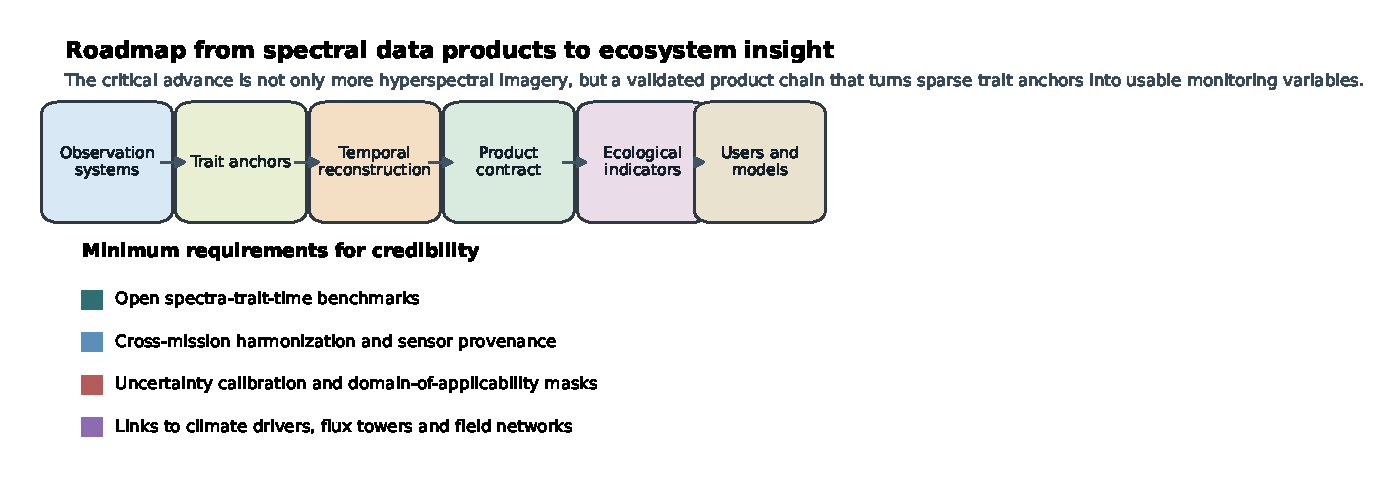
\includegraphics[width=\textwidth]{figures/generated/fig5_monitoring_roadmap.pdf}
\caption{\textbf{A roadmap for the CHIME-SBG era of functional ecosystem monitoring.} The transition from mission-driven spectral products to ecology- and climate-facing functional monitoring requires open spectra-trait-time benchmarks, cross-mission harmonization, calibrated uncertainty and domain masks, and explicit links to climate drivers, flux towers, field networks, ecosystem and Earth-system models, policymakers and user communities. The 2026--2030 window is decisive for establishing community standards before CHIME and SBG data become dominant. \textit{[Author note: figure may be updated to display an explicit 2026--2030 timeline track if NCC editors request.]}}
\label{fig:roadmap}
\end{figure}

\section{Conclusion}

The next generation of ecosystem monitoring should not ask only whether vegetation is greener or browner. It should ask which functional dimensions are changing, when they change, whether they recover and how confidently they can be interpreted. Imaging spectroscopy makes plant function observable from space, but its ecological value will depend on whether sparse observations can be transformed into continuous, validated and uncertainty-aware trait time series. Dense multispectral archives provide the temporal carrier for this transformation. The practical target is clear: monitoring systems should report trait anomalies, uncertainty, provenance and domain flags alongside greenness anomalies. The framework proposed here is testable, falsifiable and incrementally deployable: it can be built on existing PRISMA/EnMAP/EMIT data while preparing the community for the CHIME/SBG era. Doing so will move ecosystem monitoring from describing the symptoms of climate change to attributing its functional fingerprint---with the trait-level evidence that climate science increasingly demands of a warming world.

\bmhead{Acknowledgements}
Funding and project acknowledgements should be finalized before submission. Draft acknowledgement: the authors acknowledge support from the relevant MSCA and TEE Cube research context. This text should be checked against grant and journal requirements.

\bmhead{Data and code availability}
This Perspective includes an early illustration based on draft analysis outputs. Final data and code availability statements should be added once the analysis outputs and repository release are frozen.

\bibliography{references}

\end{document}
